\documentclass[UTF8]{ctexart} % 添加中文支持

% documentclass到begin之间称为导言区,可以在这里进行一些全局设置

% 使用usepackage来添加宏包
% 所谓宏包,就是一系列控制序列的合集,这些控制序列太常用,以至于人们会觉得每次将他们写在导言区太过繁琐,于是将他们打包放在同一个文件中
% 宏包就是用于拓展Latex功能的
\usepackage{graphicx} % 用于导入外部图片的宏包(推荐格式pdf>>>>png>jpg>eps)
\usepackage{amsmath} % 使用 AMS-LaTeX 提供的数学功能
\usepackage{lmodern} % 解决字体警告问题
% \usepackage[pdf]{graphviz} % graphviz绘图支持(需要安装graphviz)
% 我的评价是还不如把latex和graphviz分开使用(latex渲染,graphviz绘图,不必非得把两者合并到一起)
\usepackage{float} % 防止图片乱浮动导致图片文字顺序混乱的包
\usepackage{multirow} % 多行表格合并的宏包
\usepackage{diagbox} % 表头斜线分割宏包
\usepackage{listings} % 代码块宏包
\usepackage{color} % 颜色宏包
\usepackage{arydshln} % 表格虚线宏包
\usepackage{amssymb} % 数学符号宏包

\lstset{
    basicstyle          =   \ttfamily,          % 基本代码风格
    keywordstyle        =   \bfseries,          % 关键字风格
    commentstyle        =   \rmfamily\itshape,  % 注释的风格,斜体
    stringstyle         =   \ttfamily,  % 字符串风格
    flexiblecolumns,                % 别问为什么,加上这个
    numbers             =   left,   % 行号的位置在左边
    showspaces          =   false,  % 是否显示空格,显示了有点乱,所以不现实了
    numberstyle         =   \zihao{-5}\ttfamily,    % 行号的样式,小五号,tt等宽字体
    showstringspaces    =   false,
    captionpos          =   t,      % 这段代码的名字所呈现的位置,t指的是top上面
    frame               =   lrtb,   % 显示边框
}

\title{2018-2019编译原理卷A}
\author{Garone Lombard}
\date{\today}

\begin{document}

% 根据导言区设置生成标题、作者、日期
\maketitle % Insert the title, author and date

\newpage

\begin{abstract}
    编译原理2021-2022试卷答案自行整理
\end{abstract}

\newpage

% 生成目录(需要注意的是,目录的正确生成至少需要编译两次)
\tableofcontents

\newpage

\section{综合运用题}

\subsection{文法}

\paragraph{题干} 有文法G[E]

\begin{equation}
    \begin{aligned}
        E & \rightarrow TE+|T        \\
        T & \rightarrow FT\uparrow|F \\
        F & \rightarrow PF*|P        \\
        P & \rightarrow (E)|i
    \end{aligned}
\end{equation}

对于句型$i(E)*FT\uparrow +$,请写出其所有短语、简单短语、素短语和句柄。

\subsection{状态图}

\paragraph{题干} 有如下所示的状态图

\begin{figure}[H]
    \centering
    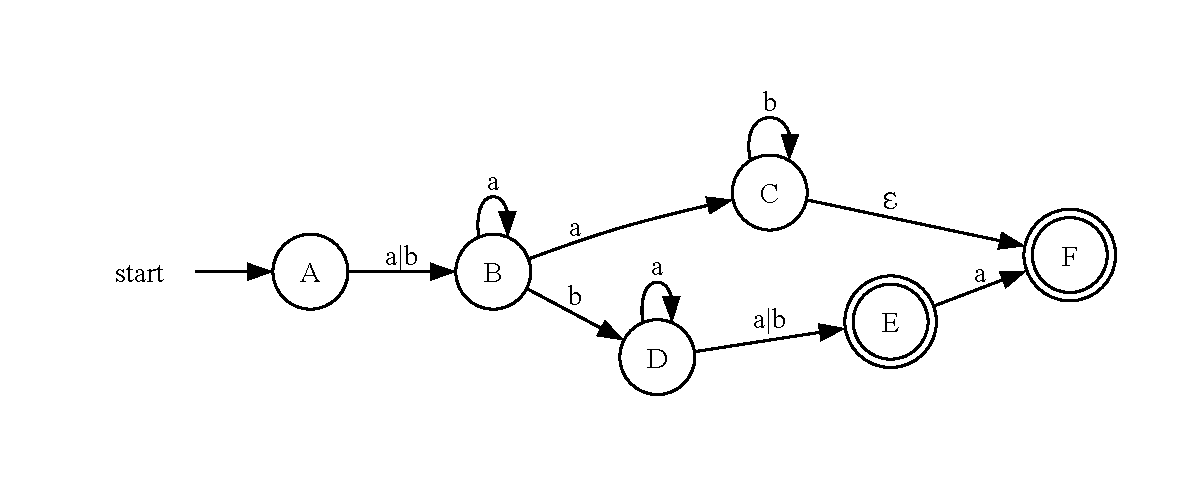
\includegraphics[width=\textwidth]{assets/nfa.pdf}
\end{figure}

\paragraph{1.} 上图所示的状态是DFA吗?如果不是,请给出原因

\paragraph{2.} 如果是DFA,则将其最小化;如果是NFA,则将其转化为DFA并最小化。

\paragraph{3.} 写出DFA M'接受的语言(正则形式)

\subsection{LL(1)文法}

\paragraph{题干} 给定文法

\begin{equation}
    \begin{aligned}
        N     & \rightarrow MN^{'}          \\
        N^{'} & \rightarrow iN|\epsilon     \\
        M     & \rightarrow PM^{'}          \\
        M^{'} & \rightarrow M|\epsilon      \\
        P     & \rightarrow QP^{'}          \\
        P^{'} & \rightarrow +P^{'}|\epsilon \\
        Q     & \rightarrow (N)|a|b|\wedge
    \end{aligned}
\end{equation}

\paragraph{1.} 求各非终结符的FIRST集和FOLLOW集

\paragraph{2.} 请说明LL(1)的充分必要条件,并判断上述文法是否为LL(1)文法

\paragraph{3.} 构造该文法的分析表,请直接填写下页表格

\begin{table}[H]
    \centering
    \begin{tabular}{|p{0.7cm}<\centering|p{0.7cm}<\centering|p{0.7cm}<\centering|p{0.7cm}<\centering|p{0.7cm}<\centering|p{0.7cm}<\centering|p{0.7cm}<\centering|p{0.7cm}<\centering|p{0.7cm}<\centering|}
        \hline
           & a & b & i & + & $\wedge$ & ( & ) & \# \\
        \hline
        N  &   &   &   &   &          &   &   &    \\
        \hline
        N' &   &   &   &   &          &   &   &    \\
        \hline
        M  &   &   &   &   &          &   &   &    \\
        \hline
        M' &   &   &   &   &          &   &   &    \\
        \hline
        P  &   &   &   &   &          &   &   &    \\
        \hline
        P' &   &   &   &   &          &   &   &    \\
        \hline
        Q  &   &   &   &   &          &   &   &    \\
        \hline
    \end{tabular}
\end{table}

\subsection{算符优先文法}

\paragraph{题干} 给定文法

\begin{equation}
    \begin{aligned}
        B & \rightarrow BoT|T      \\
        T & \rightarrow TaF|F      \\
        F & \rightarrow aF|(B)|t|f
    \end{aligned}
\end{equation}

\paragraph{1.} 什么是算符优先文法?上述文法是算符优先文法吗?

\paragraph{2.} 求各非终结符的FirstVT集和LastVT集

\paragraph{3.} 求优先关系表

\paragraph{4.} 写出句子$tafo(t)$的分析过程

\subsection{LR(1)文法}

\paragraph{题干} 有文法G[S]如下

\begin{equation}
    \begin{aligned}
        S & \rightarrow AB \\
        A & \rightarrow aB \\
        B & \rightarrow Ab \\
        B & \rightarrow b
    \end{aligned}
\end{equation}

\paragraph{1.} 求出该文法的LR(1)项目集,并构造LR(1)分析表

\paragraph{2.} 该文法是否为SLR文法,为什么?

\paragraph{3.} 利用LR(1)分析表,分析输入串aaabbbb

\subsection{存储管理}

\paragraph{题干} 有下列程序段

\begin{lstlisting}
int i1,i2;
double d3,d4;
double array1[5],array2[5][100];
int i3;
\end{lstlisting}

设整数占4个字节大小,实数占8个字节大小,起始地址为104,连续分配地址。充分利用空间不考虑对齐问题,则符号表中各标量在数据区中分配的地址为

\begin{table}[H]
    \centering
    \begin{tabular}{|p{2cm}<\centering|p{2cm}<\centering|p{2cm}<\centering|p{2cm}<\centering|}
        \hline
        名字     & 类型     & 维数 & 地址  \\
        \hline
        i1     & int    & 0  & 104 \\
        \hline
        i2     & int    &    &     \\
        \hline
        d3     & double &    &     \\
        \hline
        d4     & double &    &     \\
        \hline
        array1 & double &    &     \\
        \hline
        array2 & double &    &     \\
        \hline
        i3     & int    &    &     \\
        \hline
    \end{tabular}
\end{table}

\end{document}